\documentclass[10pt,twoside,slovak, a4paper]{article}

\usepackage[slovak]{babel}

\usepackage[IL2]{fontenc} 
\usepackage[utf8]{inputenc}
\usepackage{graphicx}
\usepackage{url} 
\usepackage{hyperref}

\usepackage{cite}

\pagestyle{headings}

\title{Koncepčné modely v hydrogeológii\thanks{Semestrálny projekt v predmete Metódy inžinierskej práce, ak. rok 2021/22, vedenie: Vladimír Mlynarovič}} 

\author{Filip Mojto\\[2pt]
	{\small Slovenská technická univerzita v Bratislave}\\
	{\small Fakulta informatiky a informačných technológií}\\
	{\small \texttt{xmojto@stuba.sk}}
	}

\date{\small 30. október 2021} 



\begin{document}


\maketitle

\begin{abstract}
Hlavným námetom na vznik tohto článku bolo opísanie súvislosti modelovania s nejakou všeobecne známou témou. Do oka nám padlo prepojenie modelovania a hydrogeológie - vednej disciplíny zaoberajúcou sa rôznymi interakciami medzi vodou, pôdou a životným prostredím. V článku preto ako prvé skúmame koncepčné modely v spojení s ich prekvapivo rozsiahlým využitím v hydrogeológii, kde môžu reprezentovať či už jednotlivé hydrogeologické celky, prípadne aj komplexný systém prúdenia podzemnej vody. Nedostatok vedomostí alebo dát môže pri procese konceptualizácie viesť k problému nazývanom „neistota pri koncepčných modeloch“. Ďalším z cieľov bolo sústredenie sa na riešenie tejto problematiky, počnúc odhalením pomocou testov a následnou elimináciou. Koncepčné modelovanie dokáže jasne a prehľadne vyobraziť rôzne merania či prieskumy dôležité pre konkrétny výskum. Náš článok sa preto zameriava aj na prezentáciu mnohých ilustrácií ako napríklad meranie interakcie dvoch podzemných vôd v hydrologickom kolektore či model lokálnej meteorickej čiary.

\ldots
\end{abstract}

\newpage

\section{Úvod}

Dôležitosť modelovania tkvie v mnohých aspektoch hydrogeológie. Najčastejšie uplatňované sú práve koncepčné modely, ktoré sa vyznačujú svojou prehľadnosťou a exaktnosťou. Časť~\ref{koncepcne} sa zaoberá dôvodmi ich využitia, ale aj nespočetnými príkladmi toho, čo môže zahŕňať pojem conceptualizácia. V neposlednom rade je v sekcii uvedené, čo všetko je potrebné na vytvorenie žiadaného modelu. Ako sa však dopracovať ku presnému modelu ? Pri uvažovaní a spracúvaní získaných dát dochádza ku kladeniu si otázok, odpovede na ne sú však často iba hypotézy. Ide o tzv. neistotu pri konceptualizácii, ktorej príčiny i následky možno nájsť vysvetlené v časti~\ref{neistota}. Jeden z následkov vedie ku vytváraniu viacerých modelov, nakoľko je nutné zobrať do úvahy všetky alternatívy. Ako sa s daným problémom čo najefektívnejšie vysporiadať je popísané v časti ~\ref{neistota:viacmodelovy}. Posledným krokom na dosiahnutie vytúženého modelu je jeho testovanie, ktoré výrazne redukuje nepresné modely, to je však len jeden z dôvodov. Podľa čoho sú modely akceptované, prípadne vylúčené, možno nájsť v časti~\ref{neistota:testovanie}.

\newpage

\section{Koncepčné modely a ich primárne využitie}\label{koncepcne}

Koncepčný model predstavuje vcelku prehľadnú reprezentáciu reality, často sa však jedná len o nejakú formu hypotézy.\cite{Tobon:CMiH} Iný zdroj charakterizuje koncečný model ako niečo, čo popisuje a kvantifikuje príslušné geologické charakteristiky, prietokové pomery, hydrobiologické procesy a mnohé iné.\cite{HC-Model} Na získanie exaktného modelu v hydrogeológii je preto nutné použiť požadované výskumné techniky v kombinácii s viacerími overovacími metódami. Samotná konštrukcia vyžaduje poznanie informácií o geologických vlastnostiach skúmaného regiónu. Dané vedomosti následne vedú k dosiahnutiu žiadeného modelu.\cite{Tobon:CMiH}. Tento proces sa dá chápať aj ako vývoj založený na dostupných geologických informáciach ako sú napríklad vodné hladiny či údaje získané zo skúšobného vrtu. Často však vychádzajú aj z bežných vedomostí, napríklad z porozumenia pre geológiu alebo z expertného výkladu.\cite{Enemark:HCMBaT}Všeobecné modelovanie má v hydrogeológii veľký význam, nakoľko slúži ako podrobná ilustrácia dôležitých hydrogeologických prvkov ako napríklad rozloženie povrchu, geometriu hydrologického kolektora, kvalitu podzemnej vody a mnohých iných. Mapy svahov, digitálnych modelov terénov a trojdimenzionálnych pohľadov reprezentujúcich topografický povrch sú získavané pomocou schopností priestorovej analýzy softwéru GIS. \cite{Tobon:CMiH}

Na obr. 1 možno vidieť príklad, ako vyzerá požadovaný koncepčný model.

\begin{figure*}[tbh]
\centering
	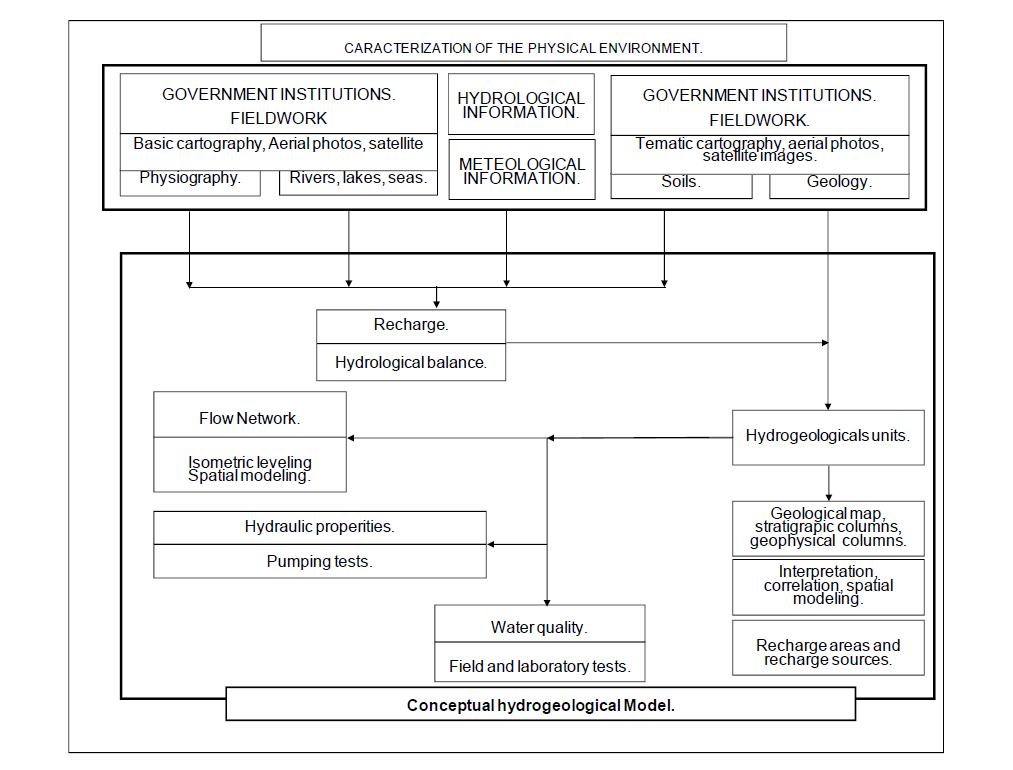
\includegraphics[width=\linewidth]{fig1.png}
	\caption{Koncepčný model\cite{Tobon:CMiH}}
	\label{Obr:1}
\end{figure*}

Ako už bolo spomenuté, hydrogeológia pracuje s koncepčnými modelmi hlavne kvôli ich prehľadnosti. Na obr. 1 je zobrazený určitý postup formou prechodov medzi stĺpcami. Ak stĺpce neoddeluje šípka prípadne medzera, tak sa jedná o istú postupnosť krokov, kde stĺpec navrchu zvyčajne vyjadruje všeobecný názov pre daný výskum a postupne sa dopracuváva až ku konkrétnym cieľom. Prvým krokom je charakterizácia fyzického prostredia, ktorá vedie k identifikácii hydrogeologických jednotiek. S danými jednotkami sa následne pracuje - zistí sa napríklad sieť toku vody, kedy sa využíva najmä priestorové modelovanie, uskutočňujú sa rôzne testy, pri ktorých sa zistí kvalita vody a mnohé ďalšie.\cite{Tobon:CMiH} 

\section{Neistota pri konceptualizácii} \label{neistota}

Koncepčný model je často označovaný ako hypotéza alebo kombinácia hypotéz, ktoré sa hromadia pri modelovaní skúmaného prostredia. Neistota pri konceptualizácii teda vzniká najmä kvôli obmedzeným údajom a vedomostiam, zvyčajne sa však s ňou počíta a je povovažaná za znížiteľnú. Nájsť pravý model môže byť náročné, nakoľko je treba otestovať mnohé interpretácie, meniacu sa zložitosť prostredia a samozrejme aj všetky zahrnuté hypotézy. Tento proces sa nazýva aj \emph{viacmodelový prístup} (\emph{multi-model approach}) (časť~\ref{neistota:viacmodelovy}). Ďalším krokom je testovanie a následná redukcia nežiadúcich modelov {časť~\ref{neistota:testovanie}.\cite{Enemark:HCMBaT}

\subsection{Viacmodelový prístup} \label{neistota:viacmodelovy}

Široká rozmanitosť aspektov, ale aj spôsob, ako vykonať rôzne konceptualizácie, vedú k vytváraniu obrovského množstva modelov, ktoré sú kvôli rýchlosti často vytvárané naraz.\cite{Enemark:HCMBaT} Tieto modely však musia spĺňať určité podmienky:

\begin{itemize}
\item Disjunktnosť a nezávislosť jeden od druhého, reprezentovatívnosť rôznych hypotéz.
\item Množstevná kompletnosť.\cite{Enemark:HCMBaT}
\end{itemize}

Množstevná kompletnosť znamená, že musí byť definovaná celá škála vierohodných koncepčných modelov, vrátane neznámych.\footnote{Koncepčné modely, ktoré aktuálne dáta ešte neobjavili, zvyčajne vedú ku koncepčným prekvapeniam.} Niektorí autori však priznávajú, že v praxi je nemožné túto podmienku naplniť.\cite{Enemark:HCMBaT} Na vytváranie alternatívnych konceptualizácií sa pracuje s tromi stratégiami:

\begin{enumerate}
\item Meniaca sa zložitosť
\item Alternatívne interpretácie
\item Testovanie hypotéz\cite{Enemark:HCMBaT}
\end{enumerate}

Príklad, ako sa testujú rôzne hypotézy, možno vidieť na obr. 2. V tomto prípade sa porovnávajú dva modely vytvorené na základe nejakých dvoch navzájom rozličných hypotéz. Rozdiel spočíva v tom, že druhá hypotéza zahŕňa do výslednej konceptualizácii údolie.

\begin{figure*}[tbh]
\centering
	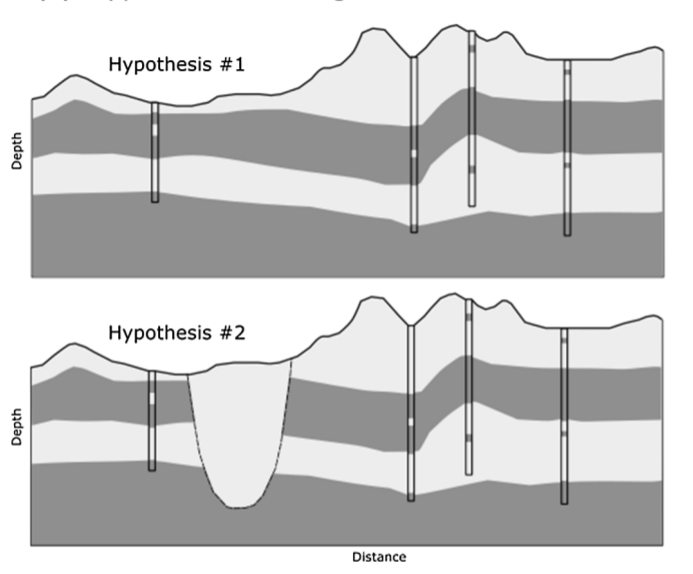
\includegraphics[width=\linewidth]{fig2.png}
	\caption{Príklad testovania dvoch rôznych hypotéz\cite{Enemark:HCMBaT}}
	\label{Obr:2}
\end{figure*}
 
\subsection{Testovanie rôznych konceptualizácií} \label{neistota:testovanie}

Keď už sú modely vytvorené, žiadúcim krokom je ich otestovanie, ktoré určuje, do akej miery sú konsistentné s príslúšnymi dátami a vedomosťami.\cite{Enemark:HCMBaT}. Testovanie je dôležité, aby sa zvýšilo porozumenie v konkrétnu problematiku a to analyzovaním a vyvracaním alternatívnych koncepčných modelov.\cite{HC-Model}  Ak si model s údajmi navzájom odporuje, je zamietnutý, alebo, lepšie povedané, pravdepodobnosť jeho presnosti sa značne znižuje. S novými údajmi však prichádzajú zmeny a niektoré zamietnuté modely sa môžu v tomto prípade stať presnými. Jestvuje preto možnosť vrátiť sa k týmto odmietnutým modelom. Všeobecne platí, že čím viac sa testuje, tým viac vzniká dôvodov pre odstránenie nepresných modelov a proces sa stáva transparentejší. Ďaľšie pozitívum, ktoré testovanie predstavuje, spočíva v odhalení neznámych modelov, čím sa predchádza vzniku koncepčných prekvapení. \cite{Enemark:HCMBaT}

\section{Koncepčné modely v praxi} \label{koncepcne modely}

\subsection{Meranie interakcie dvoch podzemných vôd} \label{koncepcne:meranie}

\subsection{Model lokálnej meteorickej čiary} \label{koncepcne:model}

\newpage

\section{Záver} \label{zaver}

\newpage

\bibliography{literatura}
\bibliographystyle{plain}
\end{document}
